\section{Supervised Learning}

\subsection{Lernprinzipien}

\begin{defi}{Ockhams Rasiermesser}
    \emph{Ockhams Rasiermesser} (Occam's Razor) bzw. das \emph{Sparsamkeitsprinzip} besagt:
    \begin{enumerate}
        \item Von mehreren möglichen hinreichenden Erklärungen für ein und denselben Sachverhalt ist die einfachste Theorie allen anderen vorzuziehen.
        \item Eine Theorie ist einfach, wenn sie möglichst wenige Variablen und Hypothesen enthält und wenn diese in klaren logischen Beziehungen zueinander stehen, aus denen der zu erklärende Sachverhalt logisch folgt.
    \end{enumerate}

    Für Machine Learning heißt das, dass Daten so einfach wie möglich erklärt bzw. modelliert werden sollten, aber nicht einfacher.
\end{defi}

\begin{bonus}{Nicht-Falsifizierbarkeit}
    Wenn das Ergebnis eines Experiments (die Daten) keine Möglichkeit hat, eine Annahme (Hypothese) zu falsifizieren, dann liefert uns das Ergebnis des Experiments (der Fit unseres Modells) keine Evidenz für oder gegen die Gültigkeit der Annahme (Hypothese).
\end{bonus}

\begin{defi}{Stichprobenverzerrung}
    Unter \emph{Stichprobenverzerrung} oder \emph{Selection Bias} versteht man die Verzerrung, die durch die Auswahl von Einzelpersonen, Gruppen oder Daten für die Analyse in einer Weise entsteht, dass keine ordnungsgemäße Randomisierung erreicht wird und somit nicht sichergestellt werden kann, dass die erhaltene Stichprobe repräsentativ für die zu analysierende Population ist.

    Der Begriff \emph{Stichprobenverzerrung} bezieht sich meist auf die Verzerrung einer statistischen Analyse, die sich aus der Methode der Stichprobenerhebung ergibt.
    Wenn der Selection Bias nicht berücksichtigt wird, können einige Schlussfolgerungen einer Annahme falsch sein.
\end{defi}

\begin{bonus}{Darstellung des Lernproblems}

    \begin{center}
        % https://tex.stackexchange.com/a/224623/243801
        \begin{tikzpicture}
            [myBox/.style={rectangle,
                        draw,
                        align=center,
                        inner sep=2.5mm}]

            \node[myBox, fill=blue!20] (unknownTargetFunction) at (-4, 4) {Unbekannte Target Function\\$f: \mathcal{X} \rightarrow \mathcal{Y}$};
            \node[myBox, fill=blue!20] (trainingExamples) at (-4, 2) {Trainingsdaten\\$\mathcal{D} = (\mathbf{x}_1,y_1),...,(\mathbf{x}_n,y_n)$};
            \node[myBox, fill=blue!20] (learningAlgorithm) at ( 0, 0) {Lernalgorithmus\\$\mathcal{A}$};
            \node[myBox, fill=blue!20] (finalHypothesis) at ( 5, 0) {Finale Hypothese\\$g \approx f$};
            \node[myBox, fill=blue!20] (hypothesisSet) at (-4,-2) {Hypothesenset\\$\mathcal{H}$};

            \node[myBox, fill=red!20] (probabilityDistribution) at (5,4) {Unbekannte\\Wahrscheinlichkeitsverteilung\\$P(\mathbf{x})$};

            \node (x) at (2, 2) {$\mathbf{x}_1, \ldots, \mathbf{x}_N$};

            \draw [->] (unknownTargetFunction) to (trainingExamples);
            \draw [->] (trainingExamples) to [bend right] (learningAlgorithm.170);
            \draw [->] (hypothesisSet) to [bend left] (learningAlgorithm.190);
            \draw [->] (learningAlgorithm) to (finalHypothesis);

            \draw [->] (probabilityDistribution) to [bend left] (x.east);
            \draw [->] (x) to (trainingExamples);
            \draw [->] (probabilityDistribution) to node [midway, right] {$\mathbf{x}$} (finalHypothesis);

            \begin{scope}[on background layer]
                \node[draw=none,opacity=.2,rounded rectangle,fill=red!50,fit=(finalHypothesis.north) (probabilityDistribution.south) (x.east)] {};
            \end{scope}

        \end{tikzpicture}
    \end{center}
\end{bonus}

\begin{defi}{Data Snooping}
    \emph{Data Snooping} ist die häufigste Falle für Machine Learning Praktiker.

    Wenn ein Datensatz den Lernprozess in irgendeiner Weise beeinflusst hat, dann wurde seine Fähigkeit zur Einschätzung der Lernleistung ($E_\text{out}$) eingeschränkt.
    \footnote{
        Man sagt auch: \enquote{Der Datensatz wurde kontaminiert.}
    }

    Zur Einschätzung der Lernleistung ($E_\text{out}$) sollte man immer einen separaten Datensatz (Testset) vorhalten, der nie für Lernentscheidungen genutzt wurde.
    Dieser soll dann zum Schluss zur Schätzung von $E_\text{out}$ eingesetzt werden.

    Typische Ursachen von Data Snooping:
    \begin{enumerate}
        \item Daten betrachten und danach sich für ein Modell entscheiden
        \item Bei der Skalierung (Vorprozessierung) von Features den gesamten Datensatz nutzen (nicht nur das Trainingset)
              \begin{itemize}
                  \item ein Fall von \emph{Data Leakage}
                  \item Informationen aus dem Testset \emph{leaken} in den Trainingset.
                  \item Best Practice:
                        \begin{itemize}
                            \item \emph{Erst} Datensatz in Training-/Validierungs-/Testset teilen
                            \item \emph{Dann} Features skalieren
                            \item Skalierung des Trainingssets auf Validierungs- und Testset anwenden
                        \end{itemize}
              \end{itemize}
        \item Denselben Datensatz immer wieder mit anderen Modellen fitten, bis $E_\text{in}$ klein wird. (Wiederverwendung derselben Daten)
        \item Stichprobenverzerrung als Konsequenz von Data Snooping
    \end{enumerate}
\end{defi}

\subsection{Logistische Regression}

\begin{defi}{Logistische Regression}
    Unter \emph{logistischer Regression} versteht man Regressionsanalysen zur Modellierung der Verteilung abhängiger diskreter Variablen.
    Wir betrachten \emph{binomiale logistische Regression} für dichotome (binäre) abhängige Variablen (Labels).

    Das logistische Regressionsmodell modelliert eine Wahrscheinlichkeit $P(y \mid \mathbf{x})$.

    Die Daten wurden durch eine uns unbekannte Target-Verteilung erzeugt:
    \[
        f(\mathbf{x}) = P(y = 1 \mid \mathbf{x})
    \]

    Das Hypothesenset $\mathcal{H}$ besteht aus Hypothesen der Form:
    \[
        h(\mathbf{x}) = \theta \left( \sum_{i=0}^d w_i x_i \right) = \theta (\mathbf{w}^T \mathbf{x}), \, \text{mit} \ \mathbf{x} \in \{1\} \times \R^d \ \text{und} \ \mathbf{w} \in \R^{d+1}
    \]
    Dabei ist $\theta(s)$ die \emph{logistische Funktion} und kann als Wahrscheinlichkeit interpretiert werden mit:
    \[
        \theta(s) = \frac{1}{1 + \exp(-s)}
    \]

    Es gilt:
    \[
        \theta(-s) = 1-\theta(s)
    \]

    % plot theta(s)
    \begin{center}
        % https://tex.stackexchange.com/a/563020/243801
        \begin{tikzpicture}[font=\sffamily]
            \begin{axis}[
                    xmin= -11,
                    xmax= 11,
                    ymin= -.1,
                    ymax= 1.1,
                    %xlabel=Modellkomplexität,
                    %ylabel=Fehler,
                    %ticks=none,
                    %xticklabels={\empty},
                    %yticklabels={\empty}
                ]
                \path[draw, dotted, thin] (axis cs:-10.0,0.0) -- (axis cs:10.0,0.0);
                \path[draw, dotted, thin] (axis cs:-10.0,1.0) -- (axis cs:10.0,1.0);

                \addplot[domain=-10:10,blue] {1/(1+e^(-x))};   %logistic function
                \node[anchor=south east,align=center] at (axis cs:6,0.8){$\theta(s)$};
                \legend{}
            \end{axis}
        \end{tikzpicture}
    \end{center}

    Die logistische Funktion ist ein Beispiel für einen \enquote{weichen Schwellenwert} (soft threshold).

    Typische Datensätze geben nicht die Wahrscheinlichkeiten vor, sondern teilen mit, ob ein Ereignis eintraf ($y = 1$) oder nicht ($y = -1$).
    Das Target ist also eine bedingte Wahrscheinlichkeit dafür, dass $y$ eintritt sofern $\mathbf{x}$ vorliegt:
    \[
        P(y \mid \mathbf{x}) = \begin{cases}
            f(x)     & \text{falls} \ y = +1 \\
            1 - f(x) & \text{falls} \ y = -1
        \end{cases}
    \]
\end{defi}

\begin{defi}{Logistisches Fehlermaß}
    Die Definition des \emph{logistischen Fehlermaßes} basiert auf dem Begriff der Likelihood:

    Wie wahrscheinlich ist es, dass wir ein Ergebnis $y$ beim Vorliegen von $\mathbf{x}$ erhalten, wenn Target $P(y \mid \mathbf{x})$ durch unsere Hypothese $h$ ausgedrückt wird?

    Es gilt (mit $h(\mathbf{x}) = \theta(\mathbf{w}^T \mathbf{x})$):
    \[
        P(y \mid \mathbf{x}) = \begin{cases}
            h(x)     & \text{falls} \ y = +1 \\
            1 - h(x) & \text{falls} \ y = -1
        \end{cases}
        = \begin{cases}
            h(x)  & \text{falls} \ y = +1 \\
            h(-x) & \text{falls} \ y = -1
        \end{cases}
        = h(y \mathbf{x}) = \theta (y \mathbf{w}^T \mathbf{x})
    \]

    Die Datenpunkte $(\mathbf{x}_1, y_1), \ldots, (\mathbf{x}_n, y_n)$ seien unabhängig voneinander generiert worden.

    Die Wahrscheinlichkeit, alle $y_i$ für gegebene $\mathbf{x}_i$ zu erhalten, ist das Produkt
    \[
        \prod_{n=1}^N P(y_n \mid \mathbf{x}_n)
    \]

    Diese Wahrscheinlichkeit soll maximiert (\emph{Maximum-Likelihood-Methode}) und darüber die finale Hypothese $h$ mit dem Gewichtsvektor $\mathbf{w}$ erhalten werden.
    Es gilt:
    \[
        \mathbf{w} = \arg\max_{\mathbf{w}} \prod_{n=1}^N P(y_n \mid \mathbf{x}_n) = \arg\min_{\mathbf{w}} -\prod_{n=1}^N P(y_n \mid \mathbf{x}_n) = \arg\min_{\mathbf{w}} \underbrace{\frac{1}{N} \sum_{n=1}^N \ln \left( 1 + e^{-y_n \mathbf{w}^T \mathbf{x}_n} \right)}_{E_\text{in}(\mathbf{w})}
    \]

    Damit erhalten wir auch den punktweisen Fehler $e_n(h(\mathbf{x}_n), y_n)$:
    \[
        e_n(h(\mathbf{x}_n), y_n) = \ln \left( 1 + e^{-y_n \mathbf{w}^T \mathbf{x}_n} \right)
    \]

    Und wie bereits definiert der In-Sample Error $E_\text{in}(\mathbf{w})$:
    \[
        E_\text{in}(\mathbf{w}) = \frac{1}{N} \sum_{n=1}^N e_n(h(\mathbf{x}_n), y_n)
    \]

    Der punktweise Fehler wird klein, wenn:
    \begin{itemize}
        \item $y_n \mathbf{w}^T \mathbf{x}_n$ groß und positiv ist $\implies \sign(\mathbf{w}^T \mathbf{x}_n) = y_n$
        \item Der Fehler wird also klein für Gewichte $\mathbf{w}$, die $\mathbf{x}_n$ richtig klassifizieren.
    \end{itemize}

    $E_\text{in}(\mathbf{w})$ ist analytisch nicht zu minimieren, stattdessen wird er numerisch minimiert.
\end{defi}

\begin{defi}{Gradientenabstieg mit fixierter Lernrate}
    Das \emph{Gradientenverfahren} wird in der Numerik eingesetzt, um allgemeine Optimierungsprobleme zu lösen.
    Dabei schreitet man (am Beispiel eines Minimierungsproblems) von einem Startpunkt aus entlang einer Abstiegsrichtung, bis keine numerische Verbesserung mehr erzielt wird.

    Wählt man als Abstiegsrichtung den negativen Gradienten, also die Richtung des lokal steilsten Abstiegs, erhält man das \emph{Verfahren des steilsten Abstiegs}.

    Vorgehen:
    \begin{enumerate}
        \item Bestimmen des Gradienten von $E_\text{in}(\mathbf{w})$ hinsichtlich $\mathbf{w}$:
              \[
                  \nabla_\mathbf{w} E_\text{in}(\mathbf{w}) = \vektor{\frac{\partial}{\partial w_0} E_\text{in}(\mathbf{w}) \\ \vdots \\ \frac{\partial}{\partial w_d} E_\text{in}(\mathbf{w})} = \nabla_\mathbf{w} \frac{1}{N} \sum_{n=1}^N \ln \left( 1 + e^{-y_n \mathbf{w}^T \mathbf{x}_n} \right) = \frac{1}{N} \sum_{n=1}^N (-y_n \mathbf{x}_n) \theta (-y_n \mathbf{w}^T \mathbf{x}_n)
              \]
        \item Wir finden numerisch das Minimum von $E_\text{in}(\mathbf{w})$ mithilfe des Gradienten mittels Gradientenabstieg:
              \begin{itemize}
                  \item Negative Gradientenrichtung führt zur stärksten Abnahme von $\Delta E_\text{in}(\mathbf{w})$:
                        \[
                            \hat{\mathbf{v}} = - \frac{\nabla E_\text{in}(\mathbf{w}(0))}{\norm{\nabla E_\text{in}(\mathbf{w}(0))}}
                        \]
                  \item Wir bewegen uns in die negative Gradientenrichtung ($\eta$ ist die Schrittweite):
                        \[
                            \mathbf{w}(t+1) = \mathbf{w}(t) + \eta \hat{\mathbf{v}}_t \qquad \text{mit} \ \hat{\mathbf{v}}_t = -\frac{\nabla E_\text{in}(\mathbf{w}(t))}{\norm{\nabla E_\text{in}(\mathbf{w}(t))}}
                        \]
                        \begin{itemize}
                            \item $\eta$ kann proportional zum Betrag des Gradienten gewählt werden:
                                  \[
                                      \eta_t = \eta \norm{\nabla E_\text{in}(\mathbf{w}(t))}
                                  \]
                            \item Damit erhalten wir einen \emph{Gradientenabstieg mit fixierter Lernrate} $\eta$:
                                  \begin{alignat*}{1}
                                      \mathbf{w}(t+1) & = \mathbf{w}(t) + \eta_t \hat{\mathbf{v}}_t                                                                                                                                       \\
                                                      & = \mathbf{w}(t) + \eta_t \left( - \frac{\nabla E_\text{in}(\mathbf{w}(t))}{\norm{\nabla E_\text{in}(\mathbf{w}(t))}} \right)                                                      \\
                                                      & = \mathbf{w}(t) + \left( \eta \norm{\nabla E_\text{in}(\mathbf{w}(t))} \right) \left( -\frac{\nabla E_\text{in}(\mathbf{w}(t))}{\norm{\nabla E_\text{in}(\mathbf{w}(t))}} \right) \\
                                                      & = \mathbf{w}(t) + \eta (-\nabla E_\text{in}(\mathbf{w}(t)))
                                  \end{alignat*}
                        \end{itemize}
              \end{itemize}
    \end{enumerate}

    Initialisierung:
    \begin{itemize}
        \item Ziehe Startgewichte $\mathbf{w}(0)$ aus Normalverteilung mit Mittelwert $0$ und kleiner Standardabweichung $\sigma$:
              \[
                  w(0)_0, \ldots, w(0)_d \sim \mathcal{N}(0, \sigma)
              \]
    \end{itemize}

    Terminierung:
    \begin{itemize}
        \item Maximale Anzahl an Iterationen $T$
        \item Fehler $E_\text{in}$ fällt unter vordefinierte Schwelle
        \item Veränderung $\Delta E_\text{in}$ kleiner als vordefinierte Schwelle
    \end{itemize}
\end{defi}

\subsection{Bäume}

\begin{defi}{Baum}
    \emph{Bäume} sind Modelle, die für Regression (\emph{Regressionsbäume}) oder für Klassifikation (\emph{Entscheidungsbäume}) genutzt werden.
    Sie sind oft einfach zu interpretieren, aber meist anderen Lernmodellen unterlegen.

    Sei $\mathbf{x} \in \mathcal{X}$ ein Feature Vector im $d$-dimensionalen Featureraum und seien $R_1, \ldots, R_M$ $M$ disjunkte Regionen (Hyperquader) des Featureraums.
    Die Hypothese $h(\mathbf{x})$ eines Baumes lautet:
    \[
        h(\mathbf{x}) = \sum_{n=1}^M c_m \mathbb{1}_m (\mathbf{x})
    \]
    \begin{itemize}
        \item $c_m$:
              \begin{itemize}
                  \item Regression: Mittelwert über alle Labels der Trainingsdatenpunkte in $R_m$
                  \item Klassifikation: Mehrheitslabel aller Trainingsdatenpunkte in $R_m$
              \end{itemize}
        \item $\mathbb{1}_m$ (Indikatorfunktion):
              \[
                  \mathbb{1}_m (\mathbf{x}) = \begin{cases}
                      1 & \text{falls} \ \mathbf{x} \in R_m    \\
                      0 & \text{falls} \ \mathbf{x} \notin R_m
                  \end{cases}
              \]
    \end{itemize}

    Die Regionen $R_1, \ldots, R_M$ werden durch \emph{rekursives binäres Teilen} (\emph{recursive binary splitting}) generiert.
    \footnote{
        Wir betrachten hier CART (Classification And Regression Trees) von Breiman et al, 1984
    }
\end{defi}

\begin{example}{Baum}
    \begin{center}
        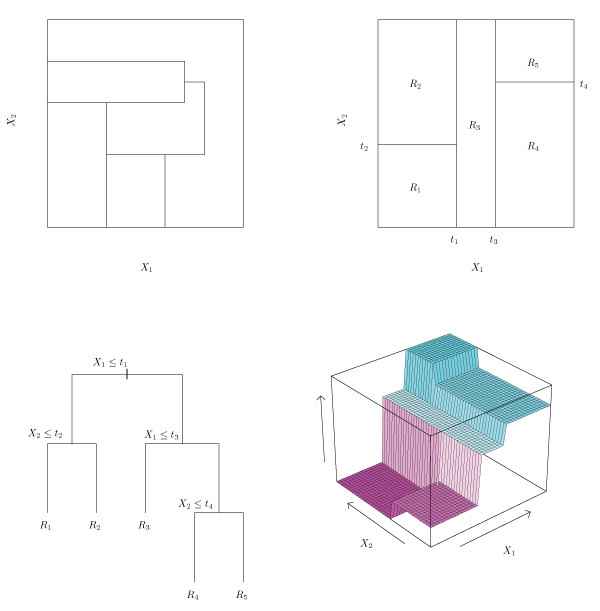
\includegraphics[width=.55\textwidth]{includes/figures/example_baeume.png}
    \end{center}

    \begin{itemize}
        \item Oben Links: Das Beispiel kann nicht durch rekursives binäres Teilen erzeugt werden.
        \item Oben Rechts: Das Beispiel kann durch rekursives binäres Teilen erzeugt werden.
        \item Unten Links: Ein Regressionsbaum, der die Partitionierung von Oben Rechts erzeugt.
        \item Unten Rechts: Ein 3D-Plot der Partitionierung von Oben Rechts.
    \end{itemize}
\end{example}

\begin{defi}{Regressionsbaum}
    Ein \emph{Regressionsbaum} soll den Featureraum $\mathcal{X}$ in $M$ disjunkte Hyperquader $R_m$ zerlegen, so dass die Werte (Labels) $y_i$ aller $\mathbf{x}_i \in R_m$ möglichst gut durch den Mittelwert $\conj{y}_m = c_m$ im Hyperquader repräsentiert werden (kleinste quadratische Abweichung zwischen $y_i$ und $y_{R_m}$).

    Das dazugehörige Optimierungsproblem ist leider nicht effizient rechnerisch lösbar:
    \[
        \min_{M, R_1, \ldots, R_M} \sum_{m=1}^M \sum_{\mathbf{x}_i \in R_m} \left( y_i - c_m \right)^2
    \]

    \emph{Greedy} Algorithmus zum lösen des Optimierungsproblems:
    \begin{enumerate}
        \item
              \begin{itemize}
                  \item Sei $R_0$ ein Hyperquader mit darin enthaltenen Trainingsdaten $(\mathbf{x}_i, y_i)$.
                  \item Sei der Featureraum $d$-dimensional, also $\mathbf{x}_i = \vektor{x_{i1}, \ldots, x_{id}}$.
                  \item Sei $j \in \{1, \ldots, d\}$ der Index eines Features.
                  \item Sei $s \in \R$ ein Schwellwert.
              \end{itemize}
        \item Definiere die Regionen
              \[
                  R_1(j, s) = \{ \mathbf{x} \mid (\mathbf{x})_j < s, \mathbf{x} \in R_0 \}
              \]
              \[
                  R_2(j, s) = \{ \mathbf{x} \mid (\mathbf{x})_j \geq s, \mathbf{x} \in R_0 \}
              \]
              Finde $(j, s)$, die die folgende Größe minimieren und damit $R_1$ und $R_2$ definieren:
              \[
                  \theta = \min_{j, s} \left( \sum_{i:x_i \in R_1 (j, s)} \left( y_i - c_1 \right)^2 + \sum_{i:x_i \in R_2 (j, s)} \left( y_i - c_2 \right)^2 \right)
              \]
              Dieser Schritt ist greedy, weil jeweils der Schnitt gewählt wird, der unmittelbar zur stärksten Abnahme von $\theta$ führt.
              %Es kann sein, dass eine bessere Partitionierung (gemäß $\theta$) in Hyperquadern existiert, diese aber nicht durch einen greedy Ansatz erreichbar ist.
        \item Für nächsten Schritt, springe zu Schritt 1, setze $R_0 = R_1$ oder $R_0 = R_2$, je nachdem, wo $\theta$ die stärkste Abnahme zeigt, oder \emph{breche ab}.
              Abbruchbedingungen können sein:
              \begin{itemize}
                  \item Jedes Blatt muss eine Mindestanzahl an Datenpunkten enthalten.
                  \item Der Baum hat eine maximal erlaubte Tiefe (\emph{tree depth}) erreicht.
                  \item Der Baum hat eine maximal erlaubte Anzahl von Blättern (\emph{tree size}) erreicht.
              \end{itemize}
    \end{enumerate}
\end{defi}

\begin{defi}{Overfitting (Regressionsbäume)}
    Mit steigender Baumtiefe wächst die Modelkomplexität und damit die Tendenz zu \emph{Overfitting}.

    Regularisierung durch \emph{Pruning}:
    \begin{itemize}
        \item \emph{Prä-Pruning Techniken}:
              \begin{itemize}
                  \item Baumwachstum wird direkt über ein Stopp-Kriterium gestoppt (z.B. Baumtiefe)
                  \item Nachteil: Eventuell werden bessere (tiefere) Teilungen verpasst.
              \end{itemize}
        \item \emph{Post-Pruning Techniken}:
              \begin{itemize}
                  \item Baum wird ausgewachsen und nachträglich gestutzt durch Entfernen (Kollabieren) von internen Knoten.
                  \item Bekannteste Methode: \emph{Cost Complexity Pruning} bzw. \emph{Weakest Link Pruning}
                        \footnote{
                            Entfernen von internen Knoten in der Reihenfolge, in der sie zum geringsten Anstieg des Vorhersagefehlers führen. Kreuzvalidierung zum Einstellen der Stärke des Prunings
                        }
              \end{itemize}
    \end{itemize}
\end{defi}

\begin{defi}{Klassifikationsbaum}
    Wir übertragen alle Überlegungen zu Regressionsbäumen auf \emph{Entscheidungsbäume} bzw. \emph{Klassifikationsbäume}, bis auf das Fehlerkriterium zum Teilen (Splitten) und Beschneiden (Prunen).

    Fehlerkriterium bei Regressionsbäumen ist der quadratischer Fehler:
    \[
        \sum_{m=1}^M \sum_{\mathbf{x}_i \in R_m} \left( y_i - c_m \right)^2
    \]

    Bei Klassifikationsproblemen markieren die Labels $y_i$ die Zugehörigkeit zu unterschiedlichen Klassen.

    Klassifikationsbäyme geben als Vorhersage die Mehrheitsklasse eines Blattes zurück.
    \footnote{
        Daher sind eindeutige Mehrheiten zu bevorzugen.
    }

    Fehlerkriterien bei Klassifikationsbäumen messen die \emph{Unreinheit} (Inhomogenität) der Blätter:
    \begin{itemize}
        \item Fehler ist 0, wenn das Blatt nur Punkte derselben Klasse enthält.
        \item Fehler ist maximal, wenn im Blatt keine Klasse eine Mehrheit hat (Patt).
    \end{itemize}
\end{defi}

\begin{defi}{Gini-Unreinheit}
    Die \emph{Gini-Unreinheit} bzw. der \emph{Gini-Index} entspricht der mittleren Wahrscheinlichkeit dsfür, dass ein zufälliger Datenpunkt falsch klassifiziert wird.

    Sei $C$ die Anzahl unterschiedlicher Klassen im Klassifikationsproblem und $p(i)$ die Wahrscheinlichkeit der Klasse $i$ in der betrachteten Datenmenge.

    Dann gilt:
    \begin{itemize}
        \item Wahrscheinlichkeit, dass ein zufälliger Datenpunkt der Klasse $i$ angehört:
              \[
                  p(i) = p_i
              \]
        \item Wahrscheinlichkeit, dass zufälliger Datenpunkt der Klasse $i$ falsch klassifiziert wird:
              \[
                  \sum_{k \neq i}^C p_k = 1 - p_i
              \]
        \item Mittlere Wahrscheinlichkeit für Falschklassifikation eines zufälligen Datenpunktes:
              \[
                  E_\text{Gini} = \sum_i^C p_i (1 - p_i) = \sum_i^C p_i - \sum_i^C p_i^2 = 1 - \sum_i^C p_i^2
              \]
    \end{itemize}

    Dabei ist:
    \begin{itemize}
        \item kleiner Gini-Index $\iff$ geringe Unreinheit
        \item größer Gini-Index $\iff$ hohe Unreinheit
    \end{itemize}

    Gini-Unreinheit wird vom Algorithmus \emph{CART} genutzt.
\end{defi}

\begin{defi}{Informationsgehalt}
    Der \emph{Informationsgehalt} $I_k$ für das Eintreffen eines Ereignisses $k$ mit Wahrscheinlichkeit $p_k$ ist:
    \[
        I_k := - \log_2 p_k \qquad (\text{Einheit: bit})
    \]

    Es gilt:
    \begin{itemize}
        \item Je seltener ein Ereignis $k$, desto größer sein Informationsgehalt.
        \item Logarithmus erleichtert das Rechnen mit Informationsgehalten.
        \item $I_k \geq 0$, da $p_k \in [0, 1]$
        \item Wahl einer anderen Basis des Logarithmus verändert nur die Einheit, in der Informationsgehalt gemessen wird
    \end{itemize}
\end{defi}

\begin{defi}{Entropie}
    Der mittlere Informationsgehalt eines Ereignisses (Ausgangs) eines Zufallsexperiments mit Zufallsvariable $X$ heißt \emph{Entropie} $H(X)$.
    \footnote{auch: Shannon-Entropie, Gibbs-Boltzmann-Entropie}

    \[
        H(X) := \Mean(I) = - \sum_{k=1}^C p_k \log_2 p_k \qquad \text{mit} \ 0 \log_2 0 = 0
    \]

    Die Entropie von $X$ unter der Bedingung des Auftretens eines Wertes $y_j$:
    \[
        H(X \mid y_j) = - \sum_{i} p(x_i \mid y_j) \log_2 p(x_i \mid y_j)
    \]
\end{defi}

\begin{defi}{Bedingte Entropie}
    Der mittlere Informationsgehalt eines Ergebnisses einer Zufallsvariablen $X$ unter der Bedingung, dass der Wert einer Zufallsvariablen $Y$ bekannt ist, heißt \emph{bedingte Entropie} $H(X \mid Y)$.
    \begin{alignat*}{1}
        H(X \mid Y) & = - \sum_{j} p(y_j) H(X \mid Y = y_j)                                              \\
                    & = - \sum_{j} p(y_j) \left( \sum_{i} p(x_i \mid y_j) \log_2 p(x_i \mid y_j) \right) \\
                    & = - \sum_{j} p(x_i, y_j) \log_2 \frac{p(x_i, y_j)}{p(y_j)}
    \end{alignat*}
\end{defi}

\begin{defi}{Information Gain}
    \emph{Information Gain} basiert auf Konzepten aus der Informationstheorie.

    Die Abnahme des mittleren Informationsgehalts eines Ergebnisses der Zufallsvariablen $X$ durch Kenntnis des Ergebnisses einer Zufallsvariablen $Y$ heißt \emph{Information Gain}.
    \[
        \IG(X, Y) = H(X) - H(X \mid Y)
    \]

    Information Gain ist auch unter der Bezeichnung \emph{Mutual information} bekannt.

    \begin{center}
        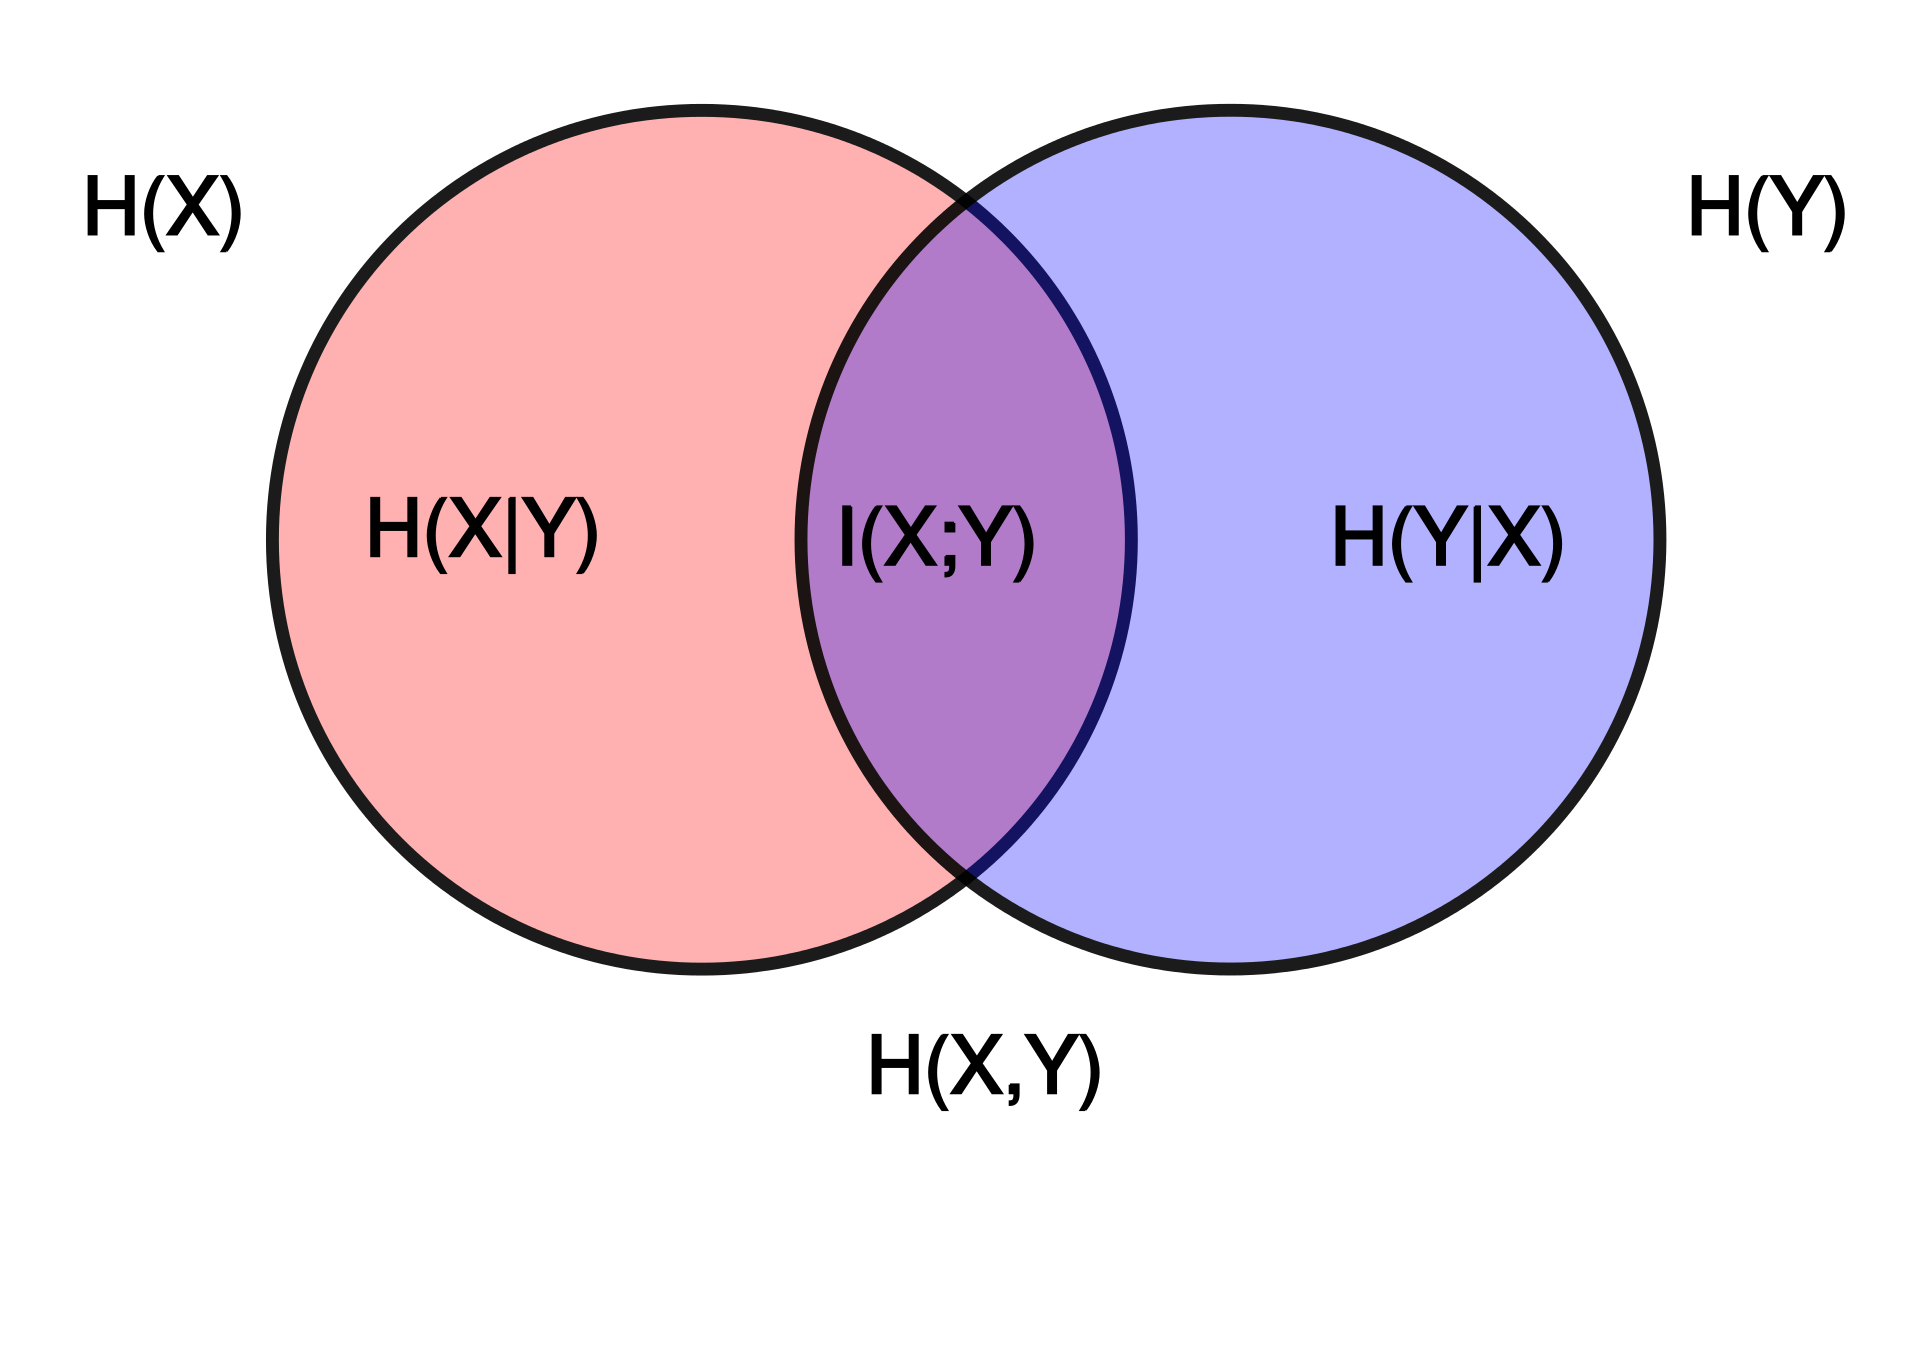
\includegraphics[width=0.7\textwidth]{includes/figures/defi_information_gain.png}
    \end{center}

    Information Gain wird von den Algorithmen \emph{ID3}, \emph{C4.5} und \emph{C5.0} genutzt.
\end{defi}

\begin{example}{Information Gain}
    \begin{center}
        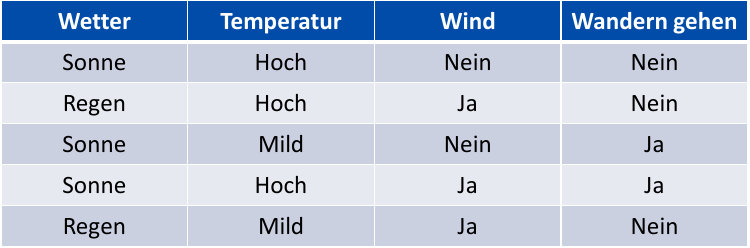
\includegraphics[width=0.6\textwidth]{includes/figures/example_information_gain.png}
    \end{center}

    % \begin{enumerate}[a)]
    %     \item Bestimmen Sie die Entropie für \enquote{Wandern gehen} (und geben Sie ihren Wert hier an).
    %     \item Bestimmen Sie die bedingten Entropien für \enquote{Wandern gehen} bezüglich der Features und geben Sie die Werte, die Sie erhalten haben, an.
    %     \item Bestimmen Sie den Information Gain für jedes Feature und geben sie die Werte hier an.
    % \end{enumerate}

    % \exampleseparator

    a) Bestimmen Sie die Entropie für \enquote{Wandern} (und geben Sie ihren Wert hier an).
    \[
        H(X) = - \sum_{k=1}^{C} p_k \log_2 p_k = - p_1 \log_2 p_1 - p_2 \log_2 p_2 = \frac{2}{5} \cdot \log_2 \frac{2}{5} - \frac{3}{5} \cdot \log_2 \frac{3}{5} \approx 0.97
    \]

    b) Bestimmen Sie die bedingten Entropien für \enquote{Wandern} bezüglich der Features und geben Sie die Werte, die Sie erhalten haben, an.
    \[
        H(Y \mid X) = - \sum_j p(x_j) \left( \sum_i p(y_i \mid x_j) \log_2 p(y_i \mid x_j) \right)
    \]

    Damit gilt:
    \[
        H(\text{Wandern} \mid \text{Wetter})
        = - \underbrace{\frac{3}{5} \left( \underbrace{\frac{2}{3} \log_2 \frac{2}{3}}_{\text{Wandern Ja}} + \underbrace{\frac{1}{3} \log_2 \frac{1}{3}}_{\text{Wandern Nein}} \right)}_{\text{Sonne}}
        - \underbrace{\frac{2}{5} \left( \underbrace{\frac{0}{2} \log_2 \frac{0}{2}}_{\text{Wandern Ja}} + \underbrace{\frac{2}{2} \log_2 \frac{2}{2}}_{\text{Wandern Nein}} \right)}_{\text{Regen}}
        \approx 0.55
    \]
    \[
        H(\text{Wandern} \mid \text{Temp.})
        = - \underbrace{\frac{3}{5} \left( \underbrace{\frac{1}{3} \log_2 \frac{1}{3}}_{\text{Wandern Ja}} + \underbrace{\frac{2}{3} \log_2 \frac{2}{3}}_{\text{Wandern Nein}} \right)}_{\text{Hoch}}
        - \underbrace{\frac{2}{5} \left( \underbrace{\frac{1}{2} \log_2 \frac{1}{2}}_{\text{Wandern Ja}} + \underbrace{\frac{1}{2} \log_2 \frac{1}{2}}_{\text{Wandern Nein}} \right)}_{\text{Mild}}
        \approx 0.95
    \]
    \[
        H(\text{Wandern} \mid \text{Wind})
        = - \underbrace{\frac{3}{5} \left( \underbrace{\frac{1}{3} \log_2 \frac{1}{3}}_{\text{Wandern Ja}} + \underbrace{\frac{2}{3} \log_2 \frac{2}{3}}_{\text{Wandern Nein}} \right)}_{\text{Wind Ja}}
        - \underbrace{\frac{2}{5} \left( \underbrace{\frac{1}{2} \log_2 \frac{1}{2}}_{\text{Wandern Ja}} + \underbrace{\frac{1}{2} \log_2 \frac{1}{2}}_{\text{Wandern Nein}} \right)}_{\text{Wind Nein}}
        \approx 0.95
    \]

    c) Bestimmen Sie den Information Gain für jedes Feature und geben sie die Werte hier an.
    \[
        \text{IG}(Y, X) = H(Y) - H(Y \mid X)
    \]

    Damit gilt:
    \[
        \text{IG}(\text{Wandern}, \text{Wetter}) = H(\text{Wandern}) - H(\text{Wandern} \mid \text{Wetter})
        = 0.97 - 0.55 = 0.42
    \]
    \[
        \text{IG}(\text{Wandern}, \text{Temperatur}) = \ldots
        = 0.97 - 0.95 = 0.02
    \]
    \[
        \text{IG}(\text{Wandern}, \text{Wind}) = \ldots
        = 0.97 - 0.95 = 0.02
    \]
\end{example}

\begin{bonus}{Gini Unreinheit vs. Information Gain}
    Welches Maß für Inhomogenität sollte für Machine Learning Projekte eingesetzt werden?

    Aus der Praxis wissen wir:
    \begin{itemize}
        \item Gini Unreinheit und Information Gain führen in knapp 2\% von Lernproblemen zu unterschiedlichen Ergebnissen.
        \item Beide Maße sind in der Praxis oft austauschbar.
    \end{itemize}

    Aus theoretischer Sicht lassen sich Gini Unreinheit und Entropie (aus der sich der Information Gain zusammensetzt) auf eine verallgemeinerte Entropie (Tsallis-Entropie) zurückführen.

    Damit sind beide Größen nah miteinander verwandt.
\end{bonus}

\begin{bonus}{Vor- und Nachteile von Bäumen}
    Vorteile:
    \begin{itemize}
        \item einfach zu erklären
        \item schnelles Training
        \item gut visualisierbar (abhängig von Baumtiefe)
        \item keine Skalierung der Features notwendig!
    \end{itemize}

    Nachteile:
    \begin{itemize}
        \item meist größere Vorhersagefehler als andere Lernmodelle
        \item starke Tendenz zum Overfitten!
    \end{itemize}
\end{bonus}

\subsection{k-Nearest Neighbors Modelle}

\begin{defi}{Ähnlichkeit}
    Es gibt sehr unterschiedliche Konzepte , um Ähnlichkeit zwischen Objekten zu quantifizieren.

    Beispiele:
    \begin{itemize}
        \item Euklidische Distanz (Unähnlichkeitsmaß):
              \[
                  d(\mathbf{x}, \mathbf{x}') = \norm{\mathbf{x} - \mathbf{x}'}
              \]
        \item Kosinus-Ähnlichkeit:
              \[
                  \CosSim(\mathbf{x}, \mathbf{x}') = \frac{\mathbf{x}^T \mathbf{x}'}{\norm{\mathbf{x}} \norm{\mathbf{x}'}}
              \]
        \item Jaccard-Koeffizient:\footnote{zur Charakterisierung der Ähnlichkeit der Mengen $S_1$ und $S_2$}
              \[
                  J(S_1, S_2) = \frac{\abs{S_1 \cap S_2}}{\abs{S_1 \cup S_2}} \in [0, 1]
              \]
    \end{itemize}
\end{defi}

\begin{defi}{Nächste Nachbarn Modelle}
    \emph{Nächste Nachbarn} (Nearest Neighbor) \emph{Modelle} zählen zu den einfachsten Machine Learning Modellen.
    Sie können je nach Problemstellung schnelle und gute Vorhersagen liefern und kommen öfters zum Einsatz zur Schätzung einer Baseline.

    Typische Modelle sind:
    \begin{itemize}
        \item Nearest Neighbor (NN)
        \item k-Nearest Neighbors (kNN Klassifikation)
        \item k-Nearest Neighbors (kNN Regression)
    \end{itemize}
\end{defi}

\begin{defi}{Nearest Neighbor}
    Seien ein Trainingsset $\mathcal{D} = (\mathbf{x}_1, y_1), \ldots, (\mathbf{x}_n, y_n)$ und ein Ähnlichkeits- bzw. Distanzmaß\footnote{Hier: Euklidische Distanz.} $d(\mathbf{x}, \mathbf{x}')$ gegeben.

    Wir betrachten einen beliebigen Punkt $\mathbf{x}$ im Featureraum:
    Die Featurevektoren $\mathbf{x}_i$ des Trainingssets liegen gemäß $d$ in unterschiedlichen Abständen zu $\mathbf{x}$.

    Die Feature Vectors des Trainingssets seien nun benannt nach ihrer Nähe zu $\mathbf{x}$:
    \begin{itemize}
        \item $\mathbf{x}_{[1]}$ bezeichne den nächsten Nachbarn von $\mathbf{x}$
        \item $\mathbf{x}_{[2]}$ bezeichne den zweitnächsten Nachbarn von $\mathbf{x}$
        \item $\ldots$
    \end{itemize}

    \[
        d(\mathbf{x}, \mathbf{x}_{[1]}) \leq d(\mathbf{x}, \mathbf{x}_{[2]}) \leq \ldots \leq d(\mathbf{x}, \mathbf{x}_{[N]})
    \]

    Die finale Hypothese des Nearest Neighbor Modells lautet dann:
    \[
        g(\mathbf{x}) = y_{[1]}(\mathbf{x})
    \]

    Es wird also das Label des nächsten Nachbarn $\mathbf{x}_{[1]}$ von $\mathbf{x}$ als Vorhersage für $\mathbf{x}$ verwendet.

    Es findet gar kein Training statt.
    Es gibt keine Parameter, die in eine Training bestimmt werden müssen.
    Die Daten definieren direkt das Modell.

    Nearest Neighbor ist ein Beispiel für \emph{instance-based learning}.
    Hypothesen solcher Modelle sind direkt durch die Trainingsdaten (Instanzen) definiert.

    Das Nearest Neighbor Modell kann bei steigender Datenpunktanzahl zu sehr komplexen Entscheidungsgrenzen führen.

    \emph{Wichtig}: Skalierung der Daten beeinflusst Nearest Neighbor Modelle.
    Lösung dafür ist Reskalierung oder Verwenden einer anderen Ähnlichkeits- bzw. Distanzfunktion.
\end{defi}

\begin{defi}{k-Nearest Neighbors (Klassifikation)}
    Eine Verallgemeinerung des Nearest Neighbor Modells ist \emph{k-Nearest Neighbors} (k-Nächste Nachbarn).

    Sei $k \geq 1$ eine ganze Zahl und $y \in \{ -1, 1 \}$.
    Dann lautet die finale Hypothese des k-Nearest Neighbors Modells:
    \[
        g(\mathbf{x}) = \sign \left( \sum_{i=1}^k y_{[i]}(\mathbf{x}) \right)
    \]

    Es wird also das Mehrheitslabel der $k$ nächsten Nachbarn $\mathbf{x}_{[1]}, \ldots, \mathbf{x}_{[k]}$ von $\mathbf{x}$ als Vorhersage für $\mathbf{x}$ verwendet.

    Analog würde eine Mehrklassen-Klassifikation mit kNN funktionieren.
\end{defi}

\begin{defi}{k-Nearest Neighbors (Regression)}
    Bei der k-Nearest Neighbors-Regression entspricht die finale Hypothese dem Mittelwert über die Labels der $k$ nächsten Nachbarn:
    \[
        g(\mathbf{x}) = \frac{1}{k} \sum_{i=1}^k y_{[i]}(\mathbf{x})
    \]
\end{defi}

\subsection{Support Vector Machine}

\begin{defi}{Support Vector Machine}
    Eine \emph{Support Vector Machine} (Stützvektormaschine) ist ein Lernmodell (also Hypothesenset und Algorithmus) und keine Machine.
    Support Vector Machines finden Hyperebenen mit \emph{breitestem Rand} (maximum margin).
    Support Vector Machines sind eine der beliebtesten \emph{Out-of-the-Box} Methoden für Klassifikationsprobleme, insbesondere da sie vielfältig einsetzbar sind.
\end{defi}

\begin{defi}{Hard Margin SVM}
    Eine \emph{Hard Margin SVM} findet die breiteste Hyperebene für linear separierbare Daten.
    \footnote{
        lineare Separierbarkeit der Daten vorausgesetzt
    }
    Dabei reduzieren breite Ränder die Modellkomplexität und damit gibt es eine Chance auf gute Generalisierung.

    Bestimmung der breitesten Hyperebene:
    \begin{enumerate}
        \item Ausgangspunkt ist das Perzeptron:
              \[
                  h(\mathbf{x}) = \sign(\mathbf{w}^T \mathbf{x})
              \]
        \item Umformulieren des Perzeptrons in eine Optimierung mit der Nebenbedingung, dass die Hyperebene den größten Rand besitzt:
              \begin{itemize}
                  \item Maximiere: $r = \frac{2}{\norm{\mathbf{w}}}$ (Breite der Margin) $\implies$ Minimiere: $\frac{1}{2} \mathbf{w}^T \mathbf{x}$
                  \item $N$ Nebenbedingungen (alle $N$ Datenpunkte richtig klassifiziert):
                        \[
                            y_n (\mathbf{w}^T \mathbf{x}_n + b) \geq 1 \qquad (n = 1, \ldots, N)
                        \]
              \end{itemize}
    \end{enumerate}

    Daraus erhält man das \emph{Duale Optimierungsproblem} der Hard Margin SVM:
    \[
        \max_\alpha \left( -\frac{1}{2} \sum_{n=1}^N \sum_{m=1}^N \left( y_n y_m \alpha_n \alpha_m \mathbf{x}^T_n \mathbf{x}_m \right) + \sum_{n=1}^N \alpha_n \right)
    \]
    unter der Nebenbedingung: $\sum_{n=1}^N \alpha_n = 0$

    Dabei gilt für den \emph{Lösungsvektor} $\vec{\alpha}$:
    \begin{itemize}
        \item Dimension von $\vec{\alpha}$ entspricht Datenpunktanzahl $N$\footnote{und hängt damit insbesondere nicht von der Dimension des Featureraums ab!}
        \item Viele Komponenten von $\vec{\alpha}$ sind $0$ (Vektor ist spärlich (sparse) besetzt)
    \end{itemize}

    Es gilt insgesamt:
    \[
        y_i = \sign \left( \sum_{n=1}^N \alpha_n y_n \mathbf{x}^T_n \mathbf{x}_i + b \right)
    \]
\end{defi}

\begin{defi}{Soft Margin SVM}
    Die \emph{Soft Margin SVM} möchte es Datenpunkten ermöglichen, den Rand einer Hard Margin SVM zu verletzten.

    Dabei stellt der Parameter $C$ den Kompromiss ein zwischen großer Breite des Randes (mit starker Verletzung, kleines $C$) und schmalem Rand (wenig Verletzung, großes $C$).

    Hier man das \emph{Duale Optimierungsproblem} der Soft Margin SVM:
    \[
        \max_\alpha \left( -\frac{1}{2} \sum_{n=1}^N \sum_{m=1}^N \left( y_n y_m \alpha_n \alpha_m \mathbf{x}^T \mathbf{x}_m \right) + \sum_{n=1}^N \alpha_n \right)
    \]
    unter den Nebenbedingungen: $\sum_{n=1}^N \alpha_n y_n = 0$, $\forall n: 0 \leq \alpha_n \leq C$

    Es gilt insgesamt:
    \[
        y_i = \sign \left( \sum_{n=1}^N \alpha_n y_n \mathbf{x}^T_n \mathbf{x}_i + b \right)
    \]
\end{defi}

\begin{defi}{Stützvektor}
    \emph{Stützvektoren} sind diejenigen Datenpunkte, die auf dem Rand der von der SVM bestimmten Hyperebene liegen oder in diese eindringen.

    Dabei gilt, dass für alle Stützvektoren $\mathbf{x}_i$ gilt:\footnote{Beweis: \href{https://stats.stackexchange.com/a/488799}{https://stats.stackexchange.com/a/488799}}
    \[
        \alpha_i \neq 0
    \]

    \begin{center}
        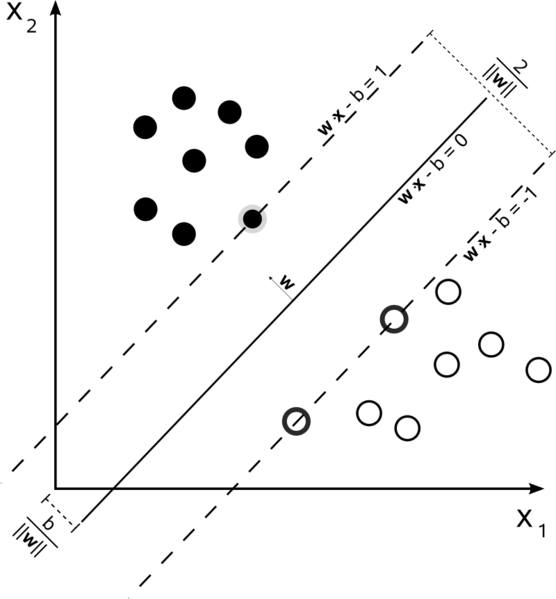
\includegraphics[width=0.5\textwidth]{includes/figures/defi_support_vector.png}
    \end{center}
\end{defi}

\begin{bonus}{Hard Margin SVM vs. Soft Margin SVM}
    Vorteile der Hard Margin SVM:
    \begin{itemize}
        \item Robuster Klassifikator bei Separierbarkeit der Daten und bei keiner bzw. geringer Rauschkontamination
    \end{itemize}

    Nachteile der Hard Margin SVM:
    \begin{itemize}
        \item Gefahr von Overfitting bei Rauschkontamination (besonders bei nichtlinearem Kernel)
    \end{itemize}
\end{bonus}

\begin{defi}{Kernel-Trick}
    Die Support Vector Machine kann als Optimierungsproblem formuliert werden.\\
    Es zeigt sich, dass alle Feature Vectors $\mathbf{x}$ nur in Skalarprodukten mit anderen auftreten.
    Daher kommt die Idee des \emph{Kernel-Tricks}:
    Kombiniere das Skalarprodukt und die nichtlineare Transformation $\Phi$ dergestalt, dass die Berechnung implizit die Featurevektoren in einen höherdimensionalen Featurespace $\mathcal{Z}$ transformiert.
\end{defi}

\begin{defi}{Polynomieller Kernel}
    Der \emph{polynomielle Kernel} enthält die polynomielle Feature-Transformation der Ordnung $Q$:
    \[
        K_\text{poly}(\mathbf{x}, \mathbf{x}') := (\zeta + \gamma \mathbf{x}^T \mathbf{x}')^Q)
    \]
    \begin{itemize}
        \item $\zeta \geq 0$: ist ein freier Parameter, der den Einfluss von Termen höherer und niedrigerer Ordnung im Polynom ausgleicht.
              %\item $\gamma$: TO DO
    \end{itemize}

    In der Praxis sind polynomielle Kernel bekannt für numerische Instabilitäten. Es ist oft schwierig, gute Parameterkombinationen $(Q, \gamma, \zeta)$ zu finden.
    Typische Wahl: $Q \leq 10$
\end{defi}

\begin{defi}{Gaußscher RBF Kernel}
    Der \emph{Gaußsche RBF Kernel} ist gebräuchlicher als der polynomielle Kernel ($\gamma = \nicefrac{1}{2\sigma^2}$):
    \footnote{
        Eine \emph{radiale Basisfunktion} (RBF) ist eine reelle Funktion $\varphi$, deren Wert nur vom Abstand zum Ursprung abhängt,  $\varphi (\mathbf {x} )=\varphi (\norm{\mathbf {x}})$.
        Der Name kommt daher, dass die Funktion nach dieser Definition radialsymmetrisch ist und ferner diese Funktionen als Basisfunktionen einer Approximation verwendet werden.
        Allgemeiner kann man den Abstand zu einem Punkt $\mathbf {c}$ betrachten, der Zentrum genannt wird, so dass $\varphi (\mathbf {x} ,\mathbf {c} )=\varphi (\norm{\mathbf {x} -\mathbf {c}})$.
    }
    \[
        K_\text{RBF}(\mathbf{x}, \mathbf{x}') := \exp(-\gamma \norm{\mathbf{x} - \mathbf{x}'}^2) = \exp \left( - \frac{\norm{\mathbf{x} - \mathbf{x}'}^2}{2\sigma^2} \right)
    \]

    \begin{center}
        % https://tex.stackexchange.com/a/563020/243801
        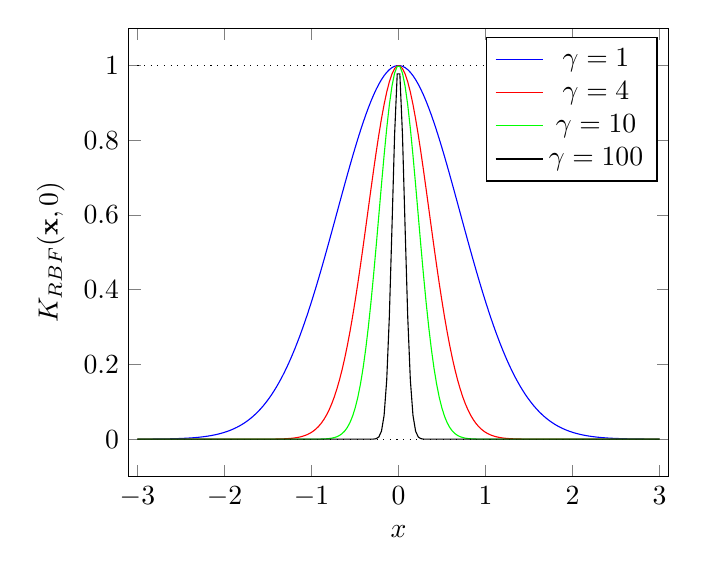
\begin{tikzpicture}[font=\sffamily]
            \begin{axis}[
                    xmin= -3.1,
                    xmax= 3.1,
                    ymin= -.1,
                    ymax= 1.1,
                    xlabel=$x$,
                    ylabel={$K_\text{RBF}(\mathbf{x}, 0)$},
                    %ticks=none,
                    %xticklabels={\empty},
                    %yticklabels={\empty}
                ]
                \path[draw, dotted, thin] (axis cs:-3.0,0.0) -- (axis cs:3.0,0.0);
                \path[draw, dotted, thin] (axis cs:-3.0,1.0) -- (axis cs:3.0,1.0);

                % gamma = 1
                \addplot[domain=-3:3,blue,samples=200] {e^(-1*(x-0)^2)};
                \addlegendentry{$\gamma=1$}
                % gamma = 4
                \addplot[domain=-3:3,red,samples=200] {e^(-4*(x-0)^2)};
                \addlegendentry{$\gamma=4$}
                % gamma = 10
                \addplot[domain=-3:3,green,samples=200] {e^(-10*(x-0)^2)};
                \addlegendentry{$\gamma=10$}
                % gamma = 100
                \addplot[domain=-3:3,black,samples=200] {e^(-100*(x-0)^2)};
                \addlegendentry{$\gamma=100$}
            \end{axis}
        \end{tikzpicture}
    \end{center}

    Dabei stellt der Parameter $\gamma$ die die Form der Hyperebenen im $\mathcal{Z}$-Raum ein.
    \begin{itemize}
        \item Große Werte für $\gamma$ führen zu komplizierten Entscheidungsgrenzen (Overfitting).
        \item Moderate Werte für $\gamma$ können zu sinnvollen Entscheidungsgrenzen führen, wobei gleichzeitig durch den maximalen Rand die Modellkomplexität regularisiert wird.
    \end{itemize}
\end{defi}

\begin{defi}{Nichtlineare Support Vector Machine}
    Für \emph{nichtlineare SVMs} gilt:
    \[
        y_i = \sign \left( \sum_{n=1}^N \alpha_n y_n \underbrace{\Phi(\mathbf{x}_n)^T \Phi(\mathbf{x}_i)}_{:= K(\mathbf{x}_n, \mathbf{x}_i)} + b \right)
    \]
    Hier wird der \emph{Kernel Trick} angewandt:
    \begin{itemize}
        \item Wir nutzen \emph{Kernel Funktionen} $K$, um das Skalarprodukt $\Phi(\mathbf{x}_n)^T \Phi(\mathbf{x}_i)$ zu ersetzen.
        \item Dadurch müssen wir nicht mehr explizit $\mathbf{x}$ nichtlinear transformieren.
        \item Nichtlineare Transformation passiert implizit im Skalarprodukt (unendlich-dimensionale Featureräume werden nun möglich).
    \end{itemize}

    Nur bestimmte Funktionen können das Skalarprodukt ersetzen.
    Es gilt die \emph{Mercer-Bedingung}:

    $K$ ist ein \emph{Kernel}, wenn die Kernelmatrix $K$ positiv semi-definit ist, wenn also für jedes $\mathbf{x}$ gilt:
    \[
        \mathbf{x}^T K \mathbf{x} \geq 0
    \]
\end{defi}

\begin{defi}{Least Squares Support Vector Machine}
    Eine \emph{Least Squares Support Vector Machine} (LS-SVM) ist eine vereinfachte Variante der SVM, die sich deutlich einfacher implementieren lässt als SVM, da nur ein lineares Gleichungssystem gelöst werden muss.

    Das \emph{Primale Optimierungsproblem} der LS-SVM ist:
    \[
        \text{Minimiere}: \frac{1}{2} \mathbf{w}^T \mathbf{w} + \frac{\gamma}{2} \sum_n e^2_n
    \]
    unter den $N$ Nebenbedingungen:
    \[
        y_n (\mathbf{w}^T \mathbf{x}_n + b) = 1 - e_n \iff y_n (\mathbf{w}^T \mathbf{x}_n + b) - 1 + e_n = 0
    \]

    Nach Umformungen ergibt sich folgendes lineare Gleichungssystem:
    \[
        \renewcommand\arraystretch{1.3}
        \left[
            \begin{array}{c|c}
                0          & \mathbf{y}^\text{T}        \\
                \hline
                \mathbf{y} & \Omega + \mathbf{I}/\gamma
            \end{array}
            \right]
        \left[
            \begin{array}{c}
                b \\
                \hline
                \vec{\alpha}
            \end{array}
            \right]
        =
        \left[
            \begin{array}{c}
                0 \\
                \hline
                \mathbf{1}
            \end{array}
            \right]
    \]

    Es ergibt sich folgendes Vorgehen:
    \begin{enumerate}
        \item Implementieren der Kernel Funktion $K$, z.B. Gaußschen RBF Kernel:
              \[
                  K(\mathbf{x}_k, \mathbf{x}_i) = \exp(-\gamma \norm{\mathbf{x}_k - \mathbf{x}_i}^2) = \exp \left( - \frac{\norm{\mathbf{x}_k - \mathbf{x}_i}^2}{2\sigma^2} \right)
              \]
        \item Bestimme die $N \times N$ Matrix
              \[
                  \Omega = \mathbf{y} \mathbf{y}^T \odot K
              \]
              \begin{itemize}
                  \item $\mathbf{y}$ ist der Labelvektor
                  \item $K$ ist die Kernelmatrix
                  \item $\odot$ ist das Hadamard-Produkt\footnote{Siehe: \href{https://de.wikipedia.org/wiki/Hadamard-Produkt}{https://de.wikipedia.org/wiki/Hadamard-Produkt}} (elementweise Multiplikation)
              \end{itemize}
        \item Bestimme die Matrix $A$:
              \[
                  A = \left[
                      \begin{array}{c|c}
                          0          & \mathbf{y}^\text{T}        \\
                          \hline
                          \mathbf{y} & \Omega + \mathbf{I}/\gamma
                      \end{array}
                      \right]
              \]
        \item Invertiere $A$ und erhalte $b$ und $\vec{\alpha}$:
              \[
                  \left[
                      \begin{array}{c}
                          b \\
                          \hline
                          \vec{\alpha}
                      \end{array}
                      \right]
                  = A^{-1}
                  \left[
                      \begin{array}{c}
                          0 \\
                          \hline
                          \mathbf{1}
                      \end{array}
                      \right]
              \]
        \item Die Vorhersage des Labels ist dann:
              \[
                  y(\mathbf{x}) = \sign \left( \sum_{k=1}^N \alpha_k y_k K(\mathbf{x}_k, \mathbf{x}) + b \right)
              \]
    \end{enumerate}
\end{defi}